\documentclass{llncs}
\usepackage[utf8x]{inputenc}
\usepackage[T1]{fontenc}
\usepackage[ngerman]{babel}
\usepackage[bookmarks=false,pagebackref,bookmarksnumbered]{hyperref}
\usepackage{pgf}
\usepackage{tikz}
\usetikzlibrary{arrows,automata}
\usepackage{multirow}
\usepackage[german]{fancyref}
\usepackage{float}
\usepackage{wrapfig}
\hyphenation{Ver-bund-wahr-schein-lich-keits-ver-tei-lung}

%opening
\title{Vergleich Probabilistischer Graphischer Modelle}
\author{Bernhard Häussner}
\institute{LS für Künstliche Intelligenz und Angewandte Informatik der Universität Würzburg}

\begin{document}

\maketitle

\begin{abstract}
In der vorliegenden Arbeit werden die Definitionen und wichtigsten Eigenschaften einiger probabilistischer graphischer Modelle (PGMs) genannt und anhand von einfachen Beispielen erklärt. Die drei Methoden bayessche Netze, naive Bayesmodelle und probabilistische Entscheidungsgraphen werden definiert und anhand einfacher Beispiele schrittweise erklärt. Im Anschluss werden Techniken zur Evaluierung solcher PGMs zusammengefasst und damit die drei verschiedenen Methoden unter Betrachtung empirischer Studien verglichen. 
\end{abstract}


\section{Einleitung}

Probabilistische graphische Modelle (PGMs) werden im Rahmen künstlicher Intelligenz interdisziplinär angewendet in vielen Bereichen, etwa Computer Vision, medizinische Entscheidungsfindung, Sprach- und Textanalyse, Zoologie und Botanik, Mikrobiologie und viele weitere. 

Während PGMs dem Anwender zu Beginn hauptsächlich in Form von Expertensystemen zur Verfügung gestellt wurden, finden sie sich heute als Anwendung für jedermann im Rahmen des Web 2.0. Hierdurch werden neue Datenquellen verarbeitet, etwa Profildaten in sozialen Netzwerken, Texte in Weblogs oder Nutzungsprofile in Onlineshops. Gewonnene Erkenntnisse können wiederum automatisiert präsentiert werden, zum Beispiel als individuelle Produktempfehlungen oder zur Filterung uninteressanter oder unerwünschter Beiträge. Beispielsweise können anhand von Twitter-Beiträgen von Benutzern, welche bekannterweise an Depression erkrankt sind, Verfahren zur Erkennung von Verhaltenssignalen für Depressionen entwickelt werden\cite{dechoudhury2013predicting}.

Ziel soll es nun sein, das Prinzip hinter verschiedenen Ansätze für PGMs verständlich zu machen. Um den Rahmen dieser Arbeit nicht zu sprengen beschränken wir uns hier auf gerichtete, diskrete PGMs, von denen drei im Folgenden genauer definiert werden. Zuletzt wird untersucht, ob alle drei Methoden in verschiedenen Einsatzszenarien ähnlich effizient und genau arbeiten. 

\section{Stochastische Grundlagen}

Um die PGMs formal beschreiben zu können und um den Kontext der hier verwendeten Notation ins Gedächtnis zu rufen, werden hier kurz einige Grundlagen definiert. Sie sind an \cite{koller2009probabilistic} orientiert. 

\subsection{Wahrscheinlichkeitsbegriff}

Wirft man eine Münze sehr häufig, so wird sich nach einer hohen Anzahl Würfen ein bestimmtes Kopf/Zahl-Verhältnis einstellen, etwa annähernd 1:1 bei einer fairen Münze, wobei die erwartete Abweichung bei mehr Würfen immer kleiner wird. Dieser Vorgang lässt sich objektiv beschreiben und in Experimenten nachvollziehen. 

Im Umfeld probabilistischer graphischer Modelle betrachtet man einen subjektiven Wahrscheinlichkeitsbegriff nach \cite{simon1958elements}. Will man beispielsweise eine Aussage über das zukünftige Wetter treffen, so kann man keine Experimente oder Stichproben durchführen. Man greift einerseits auf ein Hintergrundwissen zurück, am Beispiel Wetter wären dies die Erkenntnisse der Meteorologie, und erhält eine A-priori-Wahrscheinlichkeit. Andererseits benutzt man aktuellen Beobachtungen, etwa graue Wolken am Horizont. Formalisiert wird dies als Beobachtung oder Messwert $x$ einer Zufallsvariable $X$. Hieraus bildet man sich einen Grad persönlicher Überzeugung für ein nicht beobachtetes Phänomen, die A-posteriori-Wahrscheinlichkeitsverteilung für eine weitere Zufallsvariable $Y$, etwa ob es Regnen werde. Dieser Grad persönlicher Überzeugung ist ein Maß für die Unsicherheit. Im Beispiel wäre der Grad persönlicher Überzeugung messbar durch die festgesetzte Gewinnrate bei einer Wette, ob es Regen geben werde. 

\subsection{Zufallsvariablen}

Wir betrachten im Rahmen dieser Arbeit stets eine Menge $X_1,\dots,X_n$ diskreter Zufallsvariablen und bezeichnen eine mögliche Belegung aus dem Wertebereich von $X_i$ mit $x_i$. Die Notation $P(x_i)$ bezeichnet dabei den Grad der Überzeugung, dass $x_i$ eintritt, $P(X_i)$ die zugehörige Wahrscheinlichkeitsverteilung. Außerdem wird die Verbundwahrscheinlichkeit $P(x_i,x_k)$ und die bedingte Wahrscheinlichkeit $P(x_i,|x_k)$ jeweils auf die Wahrscheinlichkeitsverteilung erweitert als $P(X_i,X_k)$ und $P(X_i|X_k)$. 

Gilt für alle $x_i, x_k$ aus den Wertebereichen von $X_i$ und $X_k$, dass $P(x_i,x_k) = P(x_i) P(x_k)$ nennen wir die Zufallsvariablen $X_i$ und $X_k$ unabhängig und schreiben $(X_i \perp X_k)$. Zusätzlich nennen wir Variablen bedingt unabhängig, in Symbolen $(X_i \perp X_k | X_l)$, wenn stets gilt $P(x_i,x_k|x_l) = P(x_i|x_l) P(x_k|x_l)$. Dabei kann man nicht aus $(X_i \perp X_k)$ auf $(X_i \perp X_k | X_j)$ schließen. 

\paragraph{Beispiel für Zufallsvariablen} Ich werde sämtliche Beispiele an einer einfachen Menge von Zufallsvariablen erläutern, welche an der Beobachtung von Pilzarten ausgerichtet sind. Es sind dies Farbe, Muster und Gift, abgekürzt mit $F,M,G$. Sie haben die Wertebereiche "`braun"', "`rot"' für Farbe, "`keines"', "`weiße Tupfen"' für Muster und "`ja"',"`nein"' für Gift, gegebenenfalls abgekürzt durch $b,r,k,w,j,n$. Mit diesen Zufallsvariablen lassen sich die Beispiele intuitiv verstehen, so ist beispielsweise $P(j)$ der Überzeugungsgrad, dass ein Pilz giftig ist, $P(F)$ bezeichnet die Wahrscheinlichkeitsverteilung zu den Farben des Pilzes. 

\subsection{Wahrscheinlichkeitsverteilungen}

Letztendlich werden die Elementarereignisse durch den Zustand, die Belegungen, der Zufallsvariablen charakterisiert und die Wahrscheinlichkeitsverteilung ist eine reellwertige Funktion über dem Zustandsraum der Zufallsvariablen. 

Wir werden dabei Wahrscheinlichkeitsverteilungen mit $P(X_i)$ bezeichnen, und sie als Maß über den Wertebereichen der Zufallsvariablen in der Art einer Produkt-$\sigma$-Algebra multiplizieren. Die gemeinsame Wahrscheinlichkeitsverteilung (oder Verbundwahrscheinlichkeitsverteilung) über alle Zufallsvariablen ergibt sich als $ P(X_1,X_2,\dots,X_n) = \prod_{i=1}^n P(X_i) $ genau dann, wenn die betroffenen Zufallsvariablen unabhängig sind. 
% TODO Quellen
\paragraph{Beispiel einer Verbundwahrscheinlichkeitsverteilung. } 

Für die folgenden Beispiele werde ich durchgehend die Verbundwahrscheinlichkeitsverteilung in \fref{tab:bspverbwhrv} verwenden. Sie kodiert in etwa die Information, dass rote Pilze mit weißen Flocken giftig sind und braune Pilze ohne weiße Flocken genießbar, wobei andere Merkmalkombinationen eher selten sind. 

\begin{table}[htb]
\caption{\label{tab:bspverbwhrv}Beispiel-Verbundwahrscheinlichkeitsverteilung}
\centering
\begin{tabular}{l|l|l|l}
  Farbe & Muster & Gift & Wahrscheinlichkeit \\ \hline
  \multirow{4}{*}{braun} & \multirow{2}{*}{keines}       & nein & 0,54 \\
                         &                               & ja   & 0    \\
                         & \multirow{2}{*}{weiße Tupfen} & nein & 0,03 \\
                         &                               & ja   & 0,03 \\ \hline
  \multirow{4}{*}{rot}   & \multirow{2}{*}{keines}       & nein & 0,06 \\
                         &                               & ja   & 0,06 \\
                         & \multirow{2}{*}{weiße Tupfen} & nein & 0    \\
                         &                               & ja   & 0,28 \\
\end{tabular}
\end{table}

Es ist festzustellen, dass obwohl hier nur drei Zufallsvariablen involviert sind und auch diese nur zweiwertig sind, bereits eine eher unübersichtliche Tabelle zu lesen ist. 

\section{Probabilistische Graphische Modelle}

Die eben in \fref{tab:bspverbwhrv} beispielhaft gezeigte Verbundwahrscheinlichkeitsverteilung wollen wir durch probabilistische graphische Modelle darstellen. Zunächst bemühe ich mich hier um ein Verständnis der Intuition hinter PGMs und lege dann ihre Notwendigkeit im Zusammenhang mit maschineller Verarbeitung von Verbundwahrscheinlichkeitsverteilungen dar. 

\subsection{Intuition hinter probabilistischen graphischen Modellen}

Bei der Betrachtung von Naturvorgängen oder komplexen Zusammenhängen ist es laut \cite{pearl1988probabilistic} und \cite{jensen2001bayesian} ein Anliegen der Menschen diese durch Kausalitäten zu erklären, etwa "`Wenn ein Tier ein Vogel ist, so kann es Fliegen"'. 

Solcherlei Abhängigkeiten zwischen Hypothesen und Evidenz können als graphische Diagramme dargestellt werden, zunächst in der Form von Bäumen. Formalisiert werden solche Systeme als Entscheidungsbäume oder -graphen. 

Jedoch genügt es bei vielen Anwendungen nicht, boolesche Formeln zu verwenden, da ein gewisser Grad an Unsicherheit in Betracht gezogen werden muss. Somit annotiert man die erhaltenen Graphen mit  Wahrscheinlichkeitsverteilungen, und erhält eine Datenstruktur für eine gemeinsame Wahrscheinlichkeitsverteilung, ein probabilistisches graphisches Modell. 

Oftmals werden nicht direkt beobachtbare Ursachen angenommen, etwa der Jagdtrieb eines Tiers oder ein elektrisches Feld. Solche versteckten Ursachen finden sich in naiven Bayesmodellen wieder, welche in einer Zufallsvariable Komponenten definieren, die für alle weiteren Evidenzen entscheidend sind. 

Somit orientieren sich probabilistische graphische Modelle (PGMs) im Grunde an unserem menschlichen Lernen, Wissen und Folgern, können aber von Computern auf maschinenlesbaren Daten deterministisch, objektiv und schneller angewendet werden.

Wie schon in Tabelle zur Beispielverbundwahrscheinlichkeit zu erkennen, können bei der gemeinsamen Wahrscheinlichkeitsverteilung nicht direkt Abhängigkeiten abgelesen werden. Wie wir in den nächsten Abschnitten sehen werden, ist dies bei probabilistischen graphischen Modellen anders. 

\subsection{Informationstechnologische Notwendigkeit probabilistischer graphischer Modelle}

Bei \cite{koller2009probabilistic} wird die Notwendigkeit von PGMs weiter begründet: 

In der stochastischen Wahrscheinlichkeitstheorie können Wahrscheinlichkeitsverteilungen $P(X_1,X_2,\dots,X_n)$ über "`viele"' Zufallsvariablen $X_1,X_2,\dots,X_n$ abstrakt behandelt werden. Speicherte man solch eine Wahrscheinlichkeitsverteilung jedoch als Tupel in Abhängigkeit von den Zufallsvariablen ab, ergäben sich exponentiell viele Werte, für jede mögliche Belegung der Variablen eine. Im Falle von $30$ binären Zufallsvariablen wären dies bereits $2^{30} \approx 10^9 $ Werte. 

Insbesondere wäre der benötigte Speicherplatz sehr groß und die einzelnen Wahrscheinlichkeiten mitunter sehr klein. 

Zudem hätten die Algorithmen, die auf der gesamten exponentiellen Dateneingabe arbeiten, also exponentielle Laufzeit in der Anzahl der Variablen. Dieses Problem lösen PGMs, denn sie sind eine kompaktere, deklarative Repräsentation solcher Wahrscheinlichkeitsverteilungen und bilden somit die Grundlage für viele effiziente Algorithmen.

Beim automatischen Lernen bildet man PGMs aus Stichproben solcher Wahrscheinlichkeitsverteilungen, welche empirisch erfasst wurden. Hieraus kann auf die Beschaffenheit der Testobjekte geschlossen werden. PGMs können aber auch direkt von Domainexperten erstellt werden. 

% TODO: Quelle mit Enzymen

Beim Schließen benutzt man Inferenzalgorithmen, welche für gegebene Variablenbelegungen mit einem PGM die Wahrscheinlichkeitsverteilungen für Zielvariablen berechnen. 

\paragraph{Beispiel für Inferenz} In unserer Beispielverbundwahrscheinlichkeitsverteilung aus \fref{tab:bspverbwhrv} könnten wir aus der beobachteten Farbe rot auf den Überzeugungsgrad schließen, dass der rote Pilz giftig ist:
\[P(j|r) = \frac{P(r,k,j)+P(r,w,j)}{P(r)} = \frac{0,06+0,28}{0,4} = 0,85\]

Bei der Anwendung im Rahmen eines Expertensystems würde man dieses Ergebnis so interpretieren, dass man rote Pilze besser nicht isst. 

\section{Bayessche Netze}

Bayessche Netze (BN) nach \cite{pearl1988probabilistic} und \cite{koller2009probabilistic} bieten eine kompakte Darstellung für eine zusammengesetzte Wahrscheinlichkeitsverteilung über eine Menge von Zufallsvariablen als kreisfreier, gerichteter Graph, in dem bedingte Unabhängigkeiten zwischen den Variablen ablesbar sind. 

\subsection{Beschreibung}

Im Graphen stehen die Knoten für die Zufallsvariablen und die Kanten für Abhängigkeiten zwischen diesen oder die Absenz von Kanten für deren Unabhängigkeit. Die bedingten Unabhängigkeiten sind im Graph so kodiert, dass für alle $i \in \{1,\dots,n\}$ die folgende bedingte Unabhängigkeit gilt:
\[ ( X_i \perp \mbox{Nondesc}(X_i) | \mbox{Parents}(X_i) )\]
wobei $\mbox{Parents}(X_i)$ die Eltern des Knotens $X_i$ im Graphen sind und $\mbox{Nondesc}(X_i)$ jene Knoten, die keine Nachkommen des Knotens $X_i$ sind, also zu denen kein gerichteter Pfad von $X_i$ aus existiert. 

Zu jedem Knoten gehört eine bedingte Wahrscheinlichkeitsverteilung, welche die Wahrscheinlichkeiten für die Werte der Zufallsvariablen in Abhängigkeit der Werte der Zufallsvariablen der Elternknoten angibt. 

Dies bedeutet, die Wahrscheinlichkeitsverteilung lässt sich wie folgt faktorisieren: 
\[ P(X_1,X_2,\dots,X_n) = \prod_{i=1}^n P(X_i | \mbox{Parents}(X_i)) \]
wobei wiederum $\mbox{Parents}(X_i)$ die Eltern des Knotens $X_i$ im Graphen sind. 

Das Schließen ist in bayesschen Netzen möglich durch verschiedenste Algorthmen, wobei \cite{dechter1996bucket} diese Algorithmen auf den vergleichsweise einfachen\footnote{"`A student was able to implement elim-bel within a few weeks of being introduced to it. "', dt.: "`Ein Studierender konnte elim-bel innerhalb weniger Wochen nach einer Einführung implementieren."', ebd.} Algorithmus "`bucket elimination"' zurückführt. 

Die Komplexität eines bayesschen Netzes kann mit der Baumweite, also der Weite der optimalen Baumzerlegung des Graphen gemessen werden. In dieser ist das Schließen in linearer Zeit möglich. 

\subsection{Beispiel}

Die in \fref{tab:bspverbwhrv} gezeigte Beispielverbundwahrscheinlichkeitsverteilung kann durch ein bayessches Netz dargestellt werden. 

Dazu überlegen wir uns zunächst die Netzstruktur. Ein Experte könnte das Netzt mit den Gedanken strukturieren, dass die verschiedenen Muster je nach Farbe unterschiedlich oft vorkommen und die Genießbarkeit anhand von Farbe und Muster festgestellt werden kann. Der entsprechende Graph dazu sähe wie in \fref{fig:bayesnetwork} aus.

\begin{figure}[htb]
\caption{\label{fig:bayesnetwork}Beispiel für ein bayessches Netz}
\centering
\begin{tikzpicture}
  %[->,>=stealth',shorten >=1pt,auto=left,every node/.style={circle,draw}]
  [scale=0.6,->,>=stealth',shorten >=1pt,auto=left,every node/.style={circle,draw}]
  \node (nf) at (2,4) {Farbe};
  \node (nm) at (6,4)  {Muster};
  \node (ng) at (4,1)  {Gift};

  \path (nf) edge (nm);
  \path (nf) edge (ng);
  \path (nm) edge (ng);

\end{tikzpicture}
\end{figure}

Weiterhin würden die Koten mit den entsprechenden bedingten Wahrscheinlichkeitsverteilungen annotiert werden. 

Für den Knoten Farbe müsste der Experte bei unbekannter Verbundwahrscheinlichkeitsverteilung die Verteilung der Farben $P(F|\emptyset) = P(F)$ abschätzen, wie in \fref{tab:nodecolor} geschehen. Da es hier keine Elternknoten gibt, ist die Verteilung nicht bedingt. Für den Knoten Muster müsste die Verteilung der Muster in Abhängigkeit der Farben bestimmt werden, $P(M|F)$, wie in \fref{tab:nodepattern} geschehen.


\begin{table}[htb]
\begin{minipage}{0.45\textwidth}
\centering
\caption{\label{tab:nodecolor}Annotation für den Knoten Farbe}
\begin{tabular}{l|l}
  braun & rot    \\ \hline
  0,6   & 0,4    \\
\end{tabular}
\end{minipage}\hfill
\begin{minipage}{0.45\textwidth}
\centering
\caption{\label{tab:nodepattern}Annotation für den Knoten Muster}
\begin{tabular}{r|l|l}
  $F$   & keines & weiße Tupfen \\ \hline
  braun &    0,9 &          0,1 \\
  rot   &    0,3 &          0,7 \\
\end{tabular}
\end{minipage}
\end{table}




Für den Knoten Gift müsste der Fachexperte angeben, wie die giftigen Pilze aussehen, $P(G|F,M)$, siehe \fref{tab:nodepoison}.


\begin{table}[htb]
\caption{\label{tab:nodepoison}Annotation für den Knoten Gift}
\centering
\begin{tabular}{rl|l|l}
  $F$   & $M$          & nein &   ja \\ \hline
  braun & keines       &  0,5 &  0,5 \\
  braun & weiße Tupfen &  1,0 &  0,0 \\
  rot   & keines       &  0,5 &  0,5 \\
  rot   & weiße Tupfen &  0,0 &  1,0 \\
\end{tabular}
\end{table}

Multipliziert man diese drei Wahrscheinlichkeitsverteilungen erhält man wieder die Verbundwahrscheinlichkeitsverteilung aus \fref{tab:bspverbwhrv} mit 
\[P(F,M,G) = P(F) P(M|F) P(G|F,M)\]
zum Beispiel ist $ P(r,w,j) = P(r) P(w|r) P(j|r,w) = 0,4 \cdot 0,7 \cdot 1,0 = 0,28 $. Durch die Faktorisierung in drei Wahrscheinlichkeitsverteilungen wurde die Semantik der Wahrscheinlichkeiten klarer hervorgehoben. 

\section{Naive Bayesmodelle}

Bei naiven Bayesmodellen\cite{lowd2005naive} (NB) konstruiert man eine unbeobachtbare Zufallsvariable $C$. Die Zustände von $C$ nennt man Klasse oder Komponente. 

\subsection{Beschreibung}

Es wird angenommen, dass in Abhängigkeit von $C$ alle Zufallsvariablen unabhängig sind. Somit entsprechen sie einem sehr einfachen baumförmigen bayesschen Netz mit $C$ als Wurzel und den übrigen Zufallsvariablen als Blättern. Leitet man aus diesem bayesschen Netz die bedingten Unabhängigkeiten ab, ergibt sich, wie erwartet, für alle Indizes $i,k \in \{1,\dots,n\}$
\[ (X_i \perp X_k | C) \]

Die Wahrscheinlichkeitsverteilung wird wie folgt faktorisiert: 
\[ P(C,X_1,X_2,\dots,X_n) = P(C) \prod_{i=1}^n P(X_i|C) \]

Insbesondere müssen wir, um von einer gegebenen Variablenbelegung $x_1,\dots,x_n$  (Beobachtungen) 
auf die Klasse $c$ zu schließen, lediglich
\[ c = \mbox{argmax}_{c' \in C} P(c') \prod_{i=1}^n P(x_i|c') \]
berechnen. Dies ist das Prinzip des naiven Bayes-Klassifikators, die Inferenz ist hier möglich in linearer Zeit der Größe des Naiven Bayesmodells. 

Es können aber auch alle (Inferenz-)Algorithmen für Bayessche Netze verwendet werden. 

\subsection{Beispiel}

Die in \fref{tab:bspverbwhrv} gezeigte Beispielverbundwahrscheinlichkeitsverteilung kann durch ein naives Bayesmodell mit der in \fref{fig:nbgraph} gezeigten Struktur modelliert werden. 

\begin{figure}[htb]
\caption{\label{fig:nbgraph}Beispiel für ein naives Bayesmodell}
\centering
\begin{tikzpicture}
  %[->,>=stealth',shorten >=1pt,auto=left,every node/.style={circle,draw}]
  [scale=0.8,->,>=stealth',shorten >=1pt,auto=left,every node/.style={circle,draw,scale=0.8}]
  \node (nc) at (2.5,2.5) {$C$};
  \node (nf) at (1,1) {Farbe};
  \node (nm) at (2.5,1)  {Muster};
  \node (ng) at (4,1)  {Gift};

  \path (nc) edge (nf);
  \path (nc) edge (ng);
  \path (nc) edge (nm);

\end{tikzpicture}
\end{figure}

Die Anzahl der Klassen und die genauen Werte können dann mit einem Lernalgorithmus anhand der Daten gelernt werden. 

\section{Probabilistische Entscheidungsgraphen}

Probabilistische Entscheidungsgraphen (engl. probabilistic decision graphs, PDG) nach \cite{bozga1999representation}, \cite{jaeger2004probabilistic} basieren nicht auf Unabhängigkeiten zwischen Zufallsvariablen sondern auf lokalen Abhängigkeiten. 

\subsection{Beschreibung}

Die Modelle bestehen aus zwei kaskadierenden Graphen: Zum einen aus einem Wald mit Knoten für die Zufallsvariablen $P(X_1,X_2,\dots,X_n)$ und baumförmigen Abhängigkeiten zwischen diesen. Die Verbundwahrscheinlichkeiten der Variablen eines zusammenhängenden Baumes in diesem Wald sind jeweils unabhängig von den Verbundwahrscheinlichkeiten der anderen Bäume. 

Zum anderen besteht das Modell aus einer Menge gewurzelter gerichteter azyklischer Graphen für jeden Baum mit Knotenmengen $V_i$ für jede Zufallsvariable $X_i$. Für jeden Knoten in $V_i$  und für jeden Nachfolger $X_l$ von $X_i$ im Wald und jeden möglichen Wert von $X_i$ gibt es genau eine Katen zu einem Knoten aus $V_l$. Hierbei können mehrere Knoten "`zusammenfallen"'. Jeder Knoten $v_{i,k} \in V_i$ wird annotiert mit einer Wahrscheinlichkeitsverteilung $P_{i,k}(X_i)$. 

Für jede Variablenbelegung $x_1, x_2, \dots, x_n$ wird jeweils ein Knoten $v_{i,k}$ aus den $V_1, \dots, V_i$ erreicht, indem man den Kanten wie bei einem herkömmlichen Entscheidungsbaum folgt. 

Für die Verbundwahrscheinlichkeitsverteilung ergibt sich dann in Abhängigkeit der Wahrscheinlichkeitsverteilungen $P_{i,k}$ der durch Variablenbelegung erreichten Knoten: 

\[P(x_1,x_2,\dots,x_n) = \prod_{i=1}^n P_{i,k}(x_i) \]

Wie schon an der Notation zu sehen, werden anders als in bayesschen Netzen Wahrscheinlichkeitsverteilungen in Abhängigkeit von bestimmten Variablenbelegungen ausgedrückt, welche Partitionen des Zustandsraums der Zufallsvariablen bilden. Gleichzeitig gibt es Unabhängigkeiten in bayesschen Netzen, die nicht in probabilistischen Entscheidungsgraphen repräsentiert werden können, die beiden Modelle sind somit inkompatibel\footnote{Es kann jedoch mit bewährten Lernalgorithmen ein intermediäres BN gelernt werden, und aus dessen Baumzerlegung ein probabilistischer Entscheidungsgraph abgeleitet werden, wie bei \cite{jaeger2006learning} demonstriert. }. 

Inferenz ist möglich in linearer Zeit der Größe des Entscheidungsgraphen. 

\subsection{Beispiel}

Die in \fref{tab:bspverbwhrv} gezeigte Beispielverbundwahrscheinlichkeitsverteilung kann durch einen probabilistischen Entscheidungsgraphen dargestellt werden. 

Hierzu muss zuerst der Wald mit den Abhängigkeiten definiert werden. Wir wählen hier einen Baum so, dass die Wahrscheinlichkeiten des Musters von der Ausprägung der Farbe abhängen und die Wahrscheinlichkeiten für Gift von den Ausprägungen von Muster und Farbe, siehe \fref{fig:pdgforest}. 

\begin{figure}[H]
\caption{\label{fig:pdgforest}Beispiel für den Abhängigkeiten-Wald eines probabilistischen Entscheidungsgraphen}
\centering
\begin{tikzpicture}
  %[->,>=stealth',shorten >=1pt,auto=left,every node/.style={circle,draw}]
  [scale=0.75,->,>=stealth',shorten >=1pt,auto=left,every node/.style={circle,draw,scale=0.9}]
  \node (nf) at (1,3) {Farbe};
  \node (nm) at (3,2)  {Muster};
  \node (ng) at (1,1)  {Gift};

  \path (nf) edge (nm);
  \path (nm) edge (ng);

\end{tikzpicture}
\end{figure}

Danach erstellen wir für diesen Baum den gewurzelten azyklischen Graphen mit den Wahrscheinlichkeiten, siehe \fref{fig:pdgdag}.

\begin{figure}[H]
\caption{\label{fig:pdgdag}Beispiel für den gewurzelten azyklischen Graphen eines probabilistischen Entscheidungsgraphen}
\centering
\begin{tikzpicture}
  [->,>=stealth',shorten >=1pt,auto=left,every node/.style={align=center}]
  \tikzstyle{every state}=[circle,draw]
  \begin{scope}
    \draw[black, dashed, thin] (10,8) rectangle (7,6);
    \fill[black] (9.5,7) node[scale=1.2] {$V_F$};
    \node[state] (f1) at (8,7) {$v_{F,1}$ \\ $0,6/0,4$};
  \end{scope}
  \begin{scope}
    \draw[black, dashed, thin] (5,3) rectangle (11,5);
    \fill[black] (8,4) node[scale=1.2] {$V_M$};
    \node[state] (m1) at (6,4) {$v_{M,1}$ \\ $0,9/0,1$};
    \node[state] (m2) at (10,4) {$v_{M,2}$ \\ $0,3/0,7$};
  \end{scope}
  \begin{scope}
    \draw[black, dashed, thin] (3,0) rectangle (13,2); 
    \fill[black] (10,1) node[scale=1.2] {$V_G$};
    \node[state] (g1) at (4,1) {$v_{G,1}$ \\ $1,0/0,0$};
    \node[state] (g2) at (8,1) {$v_{G,2}$ \\ $0,5/0,5$};
    \node[state] (g3) at (12,1) {$v_{G,3}$ \\ $0,0/1,0$};
  \end{scope}

  \path (f1) edge node {braun} (m1);
  \path (f1) edge node {rot} (m2);
  \path (m1) edge node {keines} (g1);
  \path (m1) edge node {weiße T.} (g2);
  \path (m2) edge node {keines} (g2);
  \path (m2) edge node {weiße T.} (g3);

\end{tikzpicture}
\end{figure}

Bei der Ausprägung $(r,w,j)$ würden die Knoten $v_{F,1}$, $v_{M,2}$ und $v_{G,3}$ erreicht. Daher bestimmt sich $ P(r,w,j) $ als
\[P(r,w,j) = P_{F,1}(r) P_{M,2}(w) P_{G,3}(j) = 0,4 \cdot 0,7 \cdot 1,0 = 0,28 \]

Der probabilistische Entscheidungsgraph teilt die Verbundwahrscheinlichkeit hier sehr übersichtlich auf. 

\section{Vergleich}

Nun, da wir drei Varianten von PGMs kennen gelernt haben, bietet es sich an, diese zu evaluieren und zu vergleichen. 

\subsection{Stand der Wissenschaft}

Bei \cite{heckerman1992evaluation} wurde ein Expertensystemen für medizinische Diagnosen in zwei Versionen verglichen. Die frühere Version, basierend auf naiven Bayesmodellen analysierte 47/53 Fällen richtig, die spätere Version, nun basierend auf bayesschen Netzwerken, erreichte 50/53 richtige Analysen. 

Einen weiteren Vergleich zwischen NB und BN liefert \cite{lowd2005naive}, wo 50 Datensätze, größtenteils aus \cite{bache2013machine}, zum Lernen verwendet wurden. Hier zeigte sich, dass NB diese Datensätze teils genauer, teils an­nä­hernd gleich genau abbilden konnte, jedoch Inferenz deutlich schneller realisierbar war. Auch war NB sehr leicht zu implementieren ($2500$ LOC). 

Den Vergleich mit der dritten Methode, den probabilistischen Entscheidungsgraphen, liefert \cite{nielsen2006empirical}.

\subsection{Methodik}

Wir werden uns nun den in \cite{nielsen2006empirical} vorgenommenen Vergleich näher ansehen, da er auch viele allgemein anwendbare Methoden verwendet. 

Als Testdaten für diese Studie wurden fünf repräsentative Datensätze aus dem Repositorium \cite{bache2013machine} ausgewählt mit 7 bis 23 Variablen und bis zu rund 25000 Einträgen. Die Datensätze wurden im Verhältnis 9:1 in Lern- und Vergleichsdatensammlungen partitioniert. 

Für die theoretische Genauigkeit wird die logarithmierte Likelihood-Funktion des Modells und der Datensätze benutzt. Diese wird gegen jene Größe des Modells aufgetragen, in der die Komplexität des Inferenzvorgangs linear steigt. Es entstehen SL-Kurven\footnote{SL steht für Size-Likelihood, die Größe des Modells wird gegen die Genauigkeit aufgetragen}, an denen man die Effizienz der Methoden ablesen kann. Die Entropie der Daten $H(D)$ stellt eine obere Grenze für die logarithmierte Likelihood-Funktion dar. 

Für die empirische Messung der Inferenz-Effizienz werden zufällige Inferenz-Anfragen generiert, indem eine zufällig ausgewählte Menge von Zufallsvariablen als Evidenz- und Abfragevariablen mit zufälligen Belegungen gewählt wird. Hier wird die benötigte Zeit einer ausgewählten Implementierung gemessen und die Genauigkeit wird wiederum in SL-Kurven dargestellt. 

\begin{figure}[H]
  \caption{\label{fig:datagraphs}SL-Kurven mit empirischen Daten aus \cite{nielsen2006empirical}}
  \centering
  %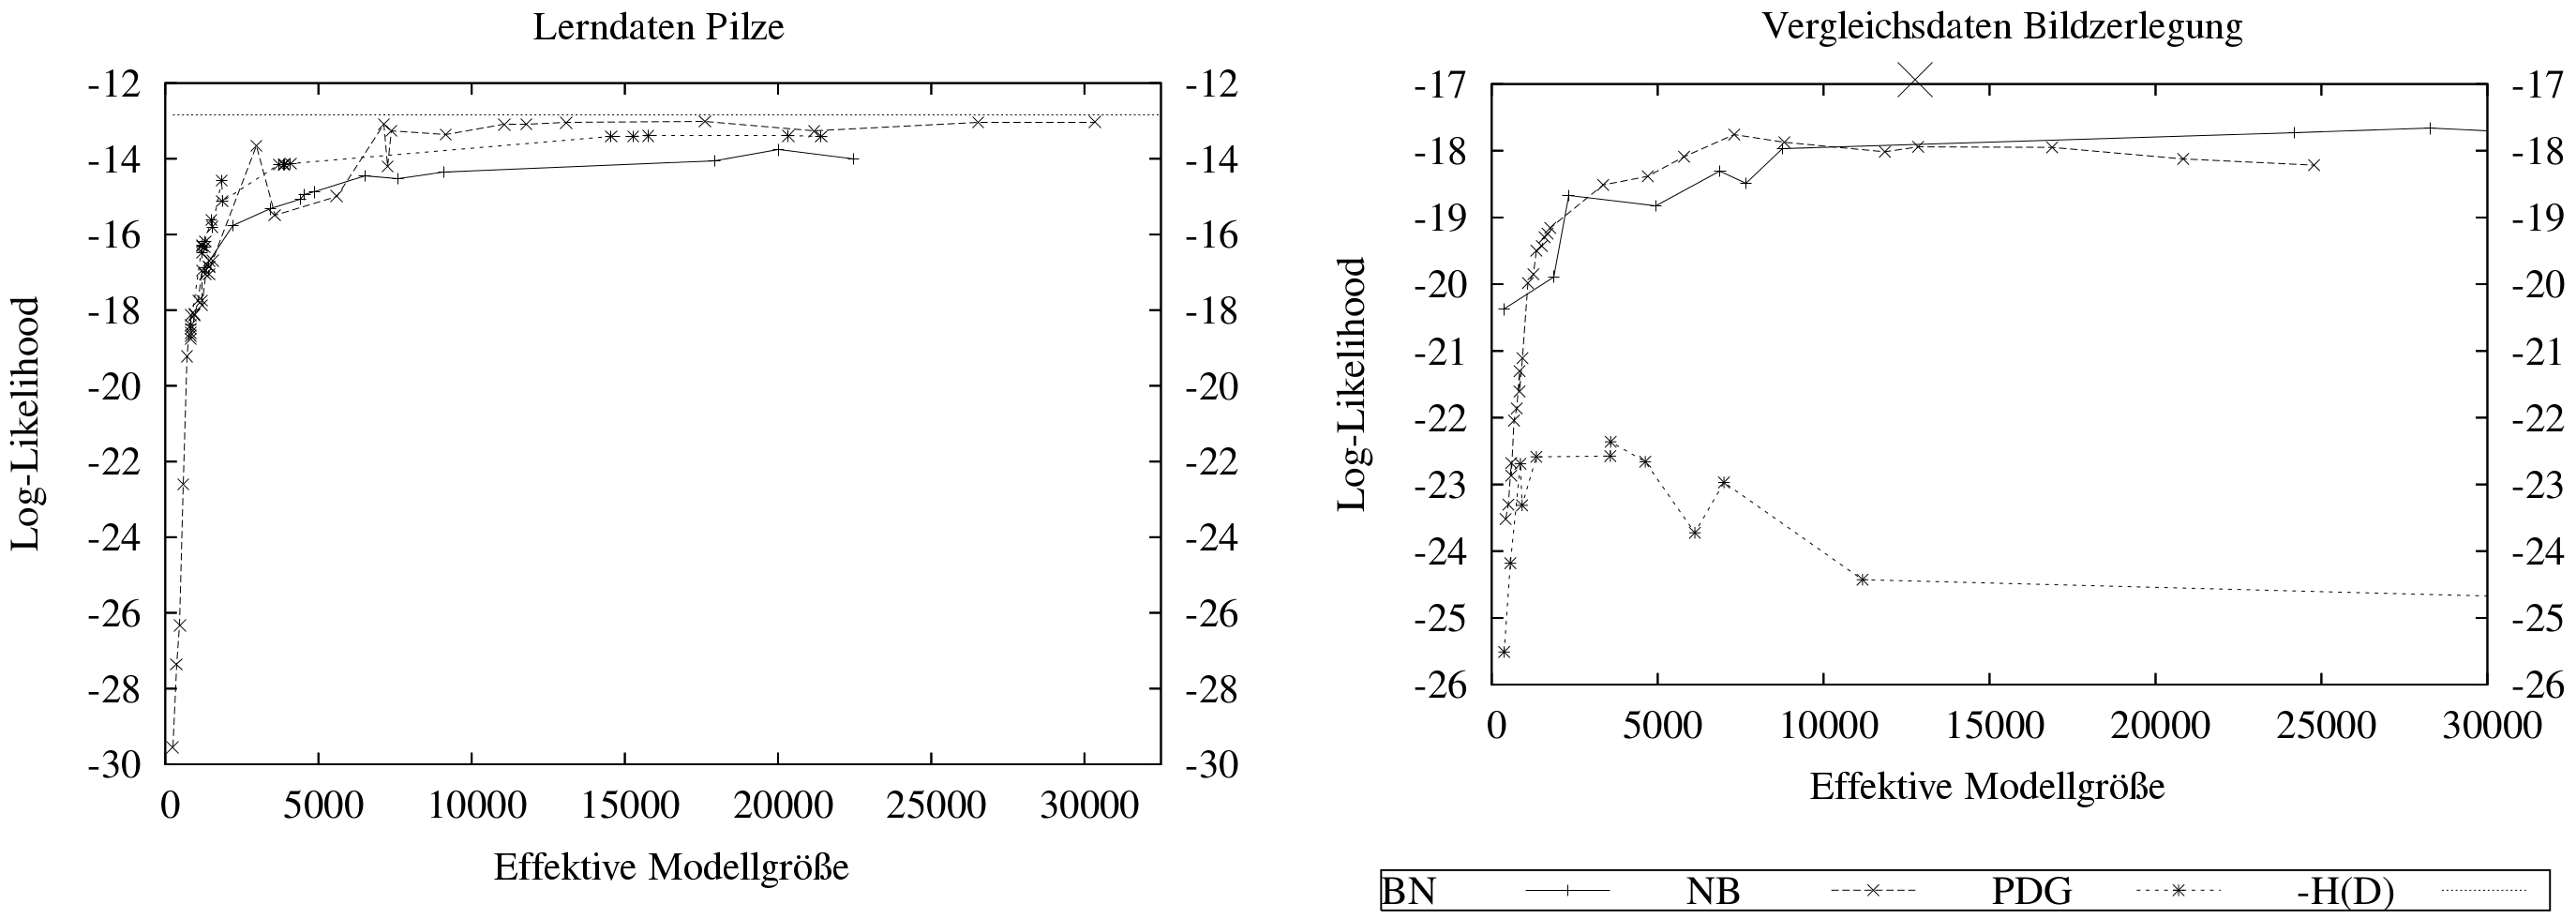
\includegraphics[width=0.7\textwidth]{graphs.png}
  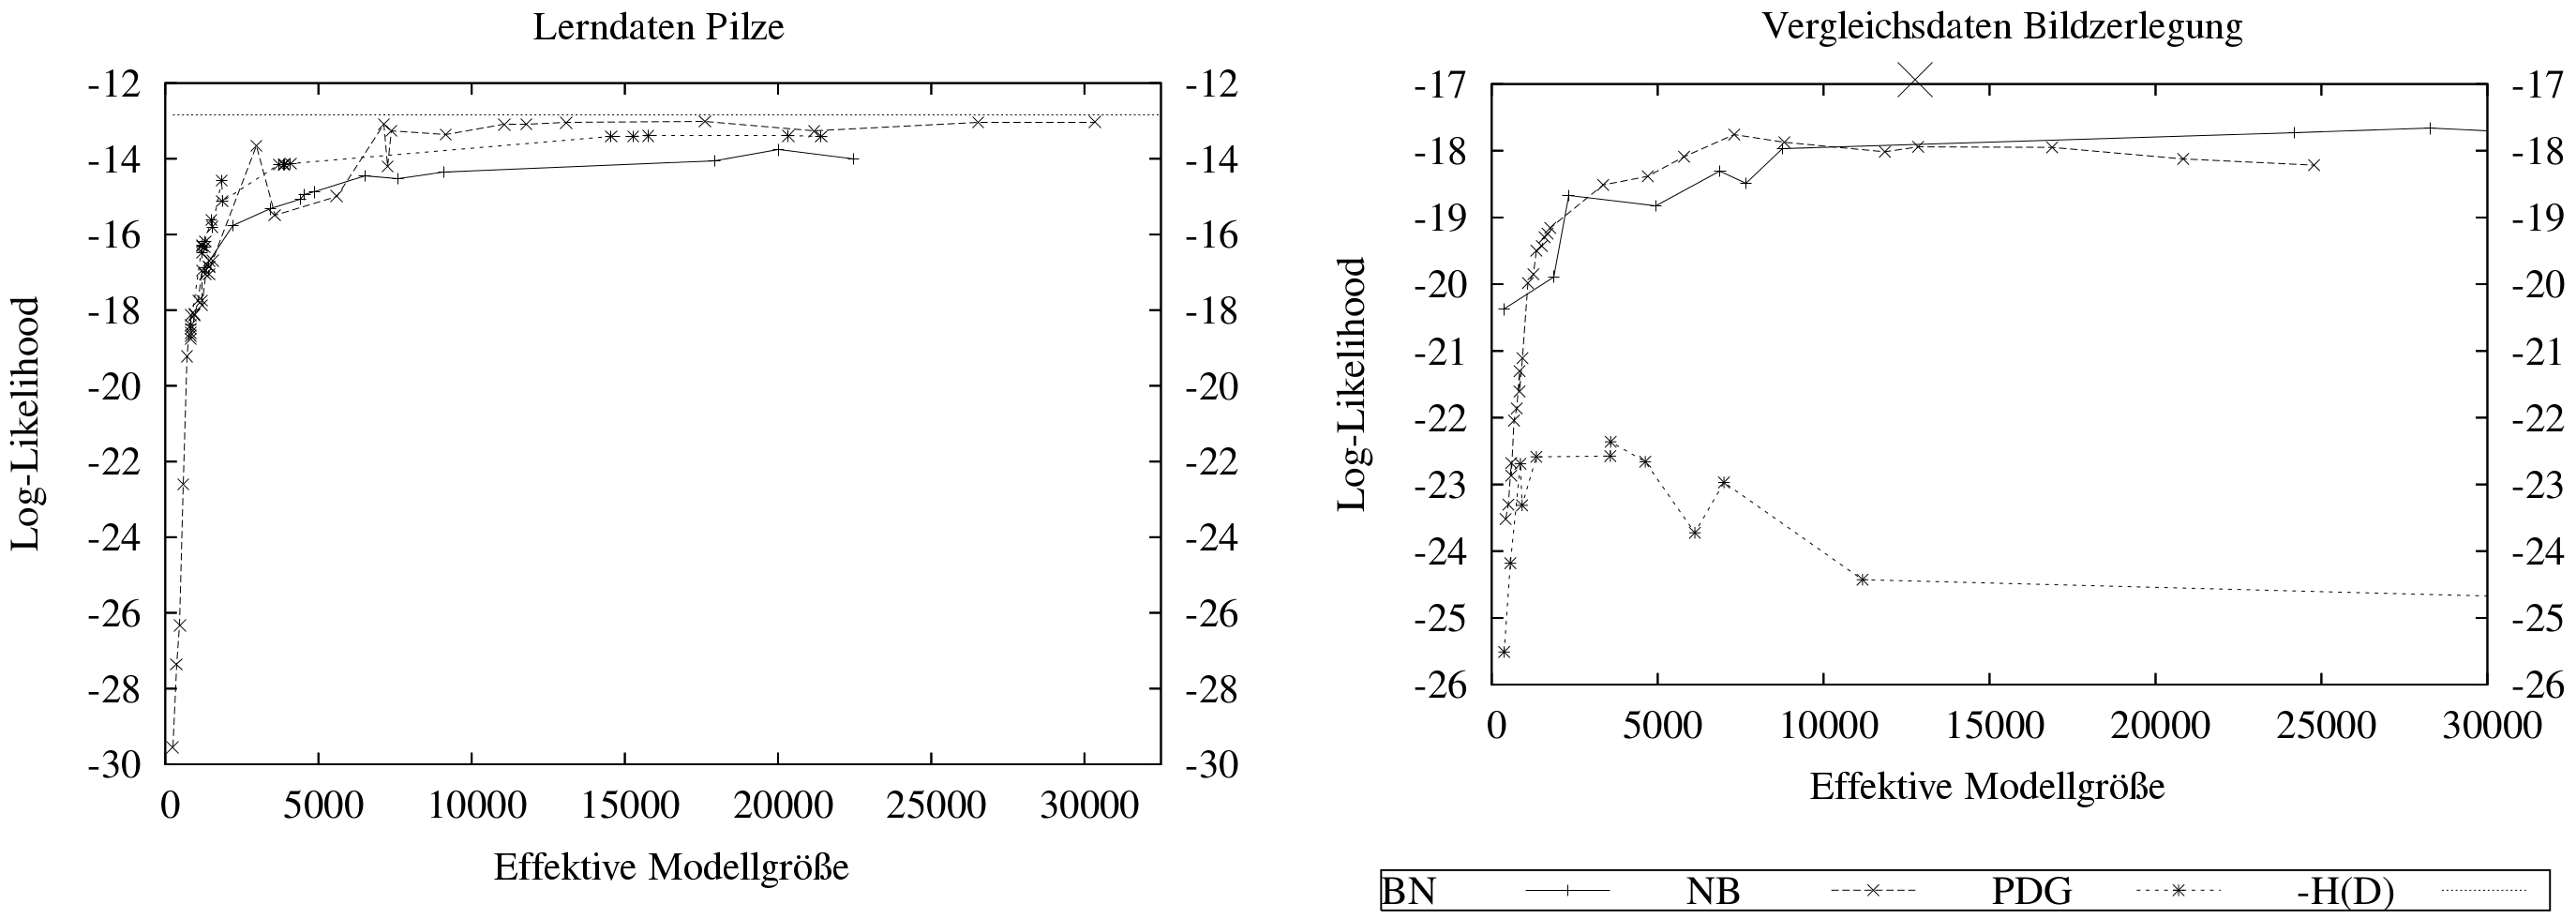
\includegraphics{graphs.png}
\end{figure}

Zwei Datensätze will ich besonders behandeln, an denen sich sehr klare Ergebnisse abzeichnen. Ihre SL-Kurven finden sich in \fref{fig:datagraphs}. 

Dies ist zum einen die Lerndatenansammlung über Pilze, in der verschiedenen Pilzarten als Tupel von 23 Eigenschaften repräsentiert werden. So kann beispielsweise der Geruch einen der Werte Mandel, Fischartig, Faulig etc. annehmen. 

Zum anderen ist dies die Vergleichsdatenansammlung aus einer Bildzerlegung von Landschaftsbildern, bei der sich für Regionen von 3x3 Pixeln jeweils die Koordinaten, durchschnittliche und extreme Farbwerte und verschiedene Maßzahlen aus (Kantenerkennungs-)Algorithmen finden. Um im diskreten zu bleiben werden die Farbwerte auf 5 Stufen quantisiert. 

\subsection{Schlussfolgerungen}

Bei der SL-Kurve für die Datenansammlung über Pilze mit rund 7500 Einträgen erkennt man, dass sich schon ab einer effektiven Modellgröße von 7500 die Log-Likelihood, also die Genauigkeit des Modells, für alle drei Methoden sehr gut ist und sich nicht mehr signifikant verbessert. Hier ist der PDG in allen Größen genauer als das BN, vielleicht ein Zeichen, dass PDGs gut geeignet sind für derartige Anwendungen. Die NB-Modelle überholen ab Größen über 7500 die anderen beiden Methoden. 

Bei der SL-Kurve für die Vergleichsdatenansammlung der Bildzerlegung ergibt sich ein durchweg schlechteres Bild für die PDGs. Dies wird damit erklärt, dass die gelernten Modelle zu nahe an den 263 Lerndateneinträgen sind, und somit nicht mehr gut auf die Fülle der rund 2000 Vergleichsdateneinträgen passen. 

Der erwartete Geschwindigkeitsvorteil von NB gegenüber BN durch die einfachere Netzstruktur konnte experimentell nicht bestätigt werden. 

Über die Gesamtheit der Graphen erkennt man, dass BN bei keinem Datensatz sehr schlechte Ergebnisse zeigte. 

\section{Zusammenfassung}

Zusammenfassend lässt sich sagen, dass keine Methode generell hinter den anderen zurück steht. Naive Bayesmodelle und probabilistische Entscheidungsgraphen lassen sich leichter implementieren und weisen oft dennoch vergleichbare Qualitäts- und Geschwindigkeits-Charakteristika wie bayessche Netze auf. Bayessche Netze konnten jedoch unabhängig von der Beschaffenheit der Daten stets akzeptable Modelle bilden. Somit empfiehlt sich eine gleichberechtigten Anwendung der drei Methoden im Bereich des Web 2.0. 

\bibliography {haeussner}
\bibliographystyle{splncs}
\end{document}
